\chapter{Weryfikacja przyjętej struktury regulatora}
\label{porownanie}
Chcąc sprawdzić jaki wpływ na działanie całego układu mają wprowadzone dodatkowe regulatory \textit{feedforward} przeprowadzono analogiczne badania symulacyjne dla układu zaprezentowanego na rysunku \ref{new_schemat}. Na potrzeby symulacji przyjęto, że obiekt sterowania będzie drugiego rzędu.\\
 W tym przypadku skupiono się głównie na analizie działania układu w następujących przypadkach:
\begin{enumerate}
	\item stabilizacja układu na poziomie 20 bez zakłóceń,
	\item działanie regulatora w sytuacji występowania zakłócenia $z_2$,
	\item działanie regulatora przy aktywnym zakłóceniu $z_1$,
	\item zachowanie się systemu w przypadku gdy oba zakłócenia są aktywne. 
\end{enumerate}
%
\begin{figure}[h!]
	\centering
	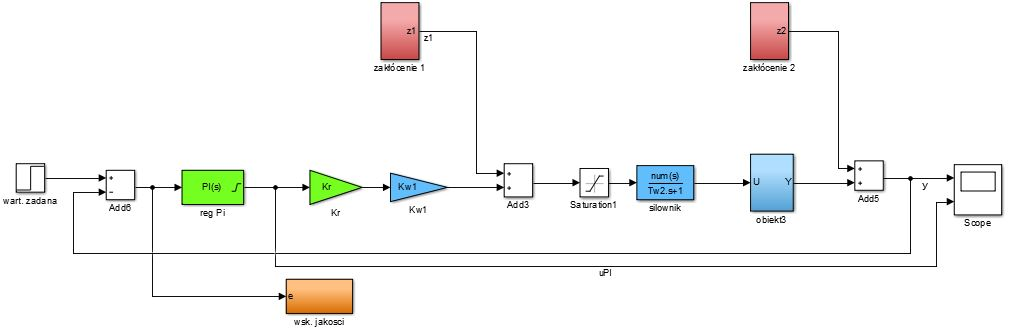
\includegraphics[scale = 0.7]{fig/model_podst.jpg}
	\caption		
	{Podstawowy model układu sterowania}
	\label{new_schemat}
\end{figure} 
%
Do optymalizacji zostały wykorzystane skrypty zamieszczone w rozdziale \ref{implementacja}. \\
Niestety procedura optymalizacji nie potrafiła znale\'zć optymalnych nastaw regulatorów dla przypadku gdy oba zakłócenia były aktywne.
W tabeli \ref{bez_feedforward_tab} zamieszczono wartości wska\'zników jakości dla każdego z przypadków.\\
\newpage
Jak można zauważyć na rysunku \ref{wykres_5} klasyczny regulator $PI$ bardzo dobrze poradził sobie z zadaniem stabilizacji na poziomie 20 bez obecność zakłóceń.W przypadku aktywacji zakłócenia $z_2$ - rysunek \ref{wykres_6}, klasyczne podejście także poradziło sobie ze zniwelowaniem niepożądanego sygnału. Dla aktywnego zakłócenia $z_1$ pojedynczy regulator $PI$ również spełnił swoje zadanie, jednak nasycanie się sygnału sterującego (rysunek \ref{wykres_7}) może zwiastować problemy ze stabilizacją dla zakłócenia o większej amplitudzie i dłuższym czasie działania.
\begin{table}[h!]
	\centering
	\caption{Wartości nastaw regulatorów oraz wska\'znika jakości dla różnych wartości zadanych i różnych zestawów zakłóceń.}
	\label{bez_feedforward_tab}
	\begin{tabular}{|c|c|c|c|c|c|c|}
		\hline
		r & z1 & z2& P3 & I3 & Kr & J \\ \hline
		20 & Nieaktywne & Nieaktywne & 0,172 & 0,074 & 0,0093 & 62,927 \\ \hline
		0 & Nieaktywne & Aktywne & 5,481 & 2,381 & 0,0003 & 30,538 \\ \hline
		0 & Aktywne & Nieaktywne & 1,798 & 0,395 & 0,0012 & 309,038 \\ \hline
	\end{tabular}
\end{table}

\begin{figure}[h!]
	\centering
	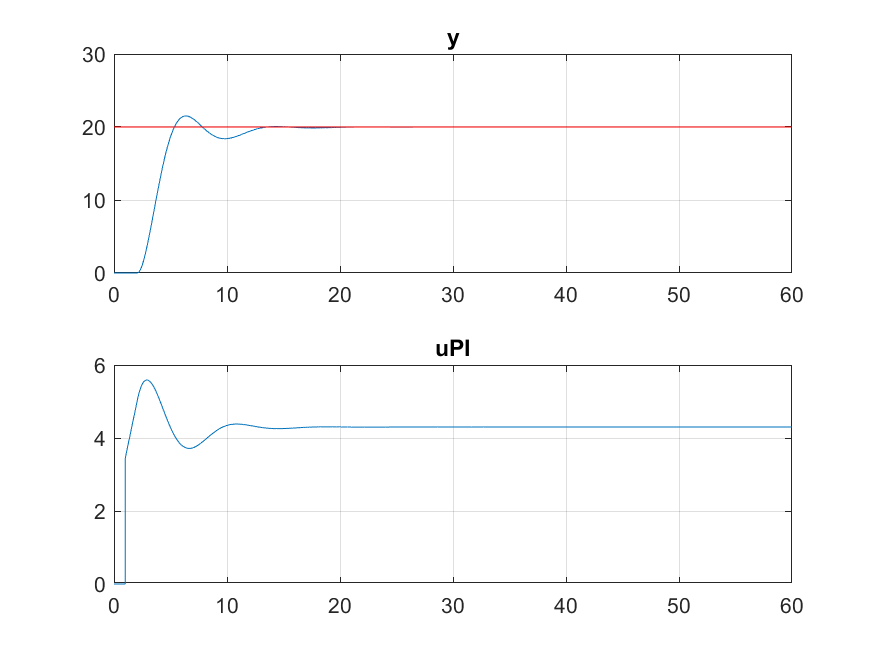
\includegraphics[scale = 0.8]{fig/bezFeedforward/fig1_2_20_bezZaklocen.png}
	\caption		
	{Odpowiedź obiektu drugiego rzędu bez regulatora feedforward, r = 20}
	\label{wykres_5}
\end{figure} 

\begin{figure}[h!]
	\centering
	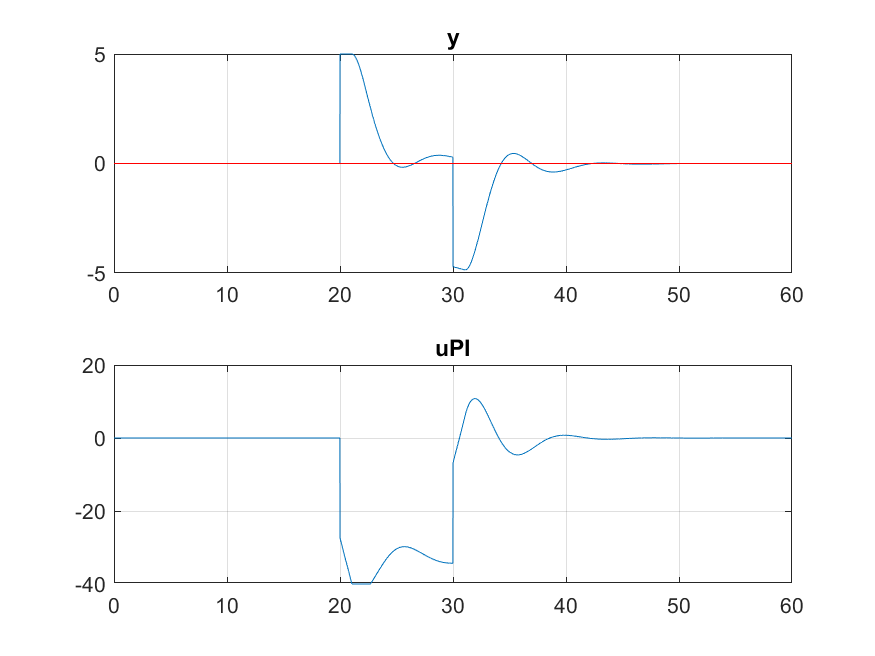
\includegraphics[scale = 0.8]{fig/bezFeedforward/fig1_2_0_z2.png}
	\caption		
	{Odpowiedź obiektu drugiego rzędu bez regulatora feedforward, r = 0, aktywne zakłócenie $z_2$}
	\label{wykres_6}
\end{figure}

\begin{figure}[h!]
	\centering
	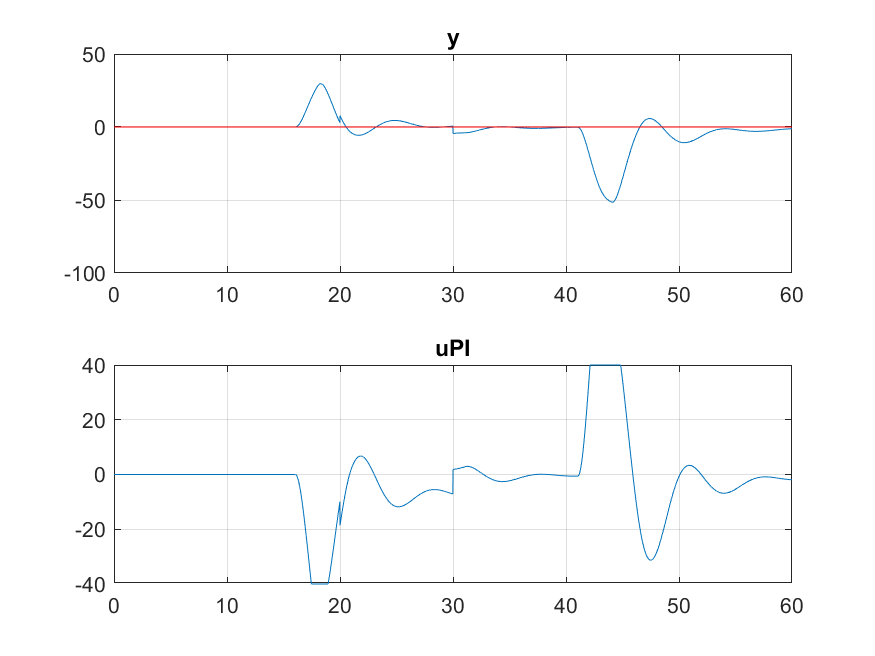
\includegraphics[scale = 0.8]{fig/bezFeedforward/fig1_2_0_z1z2.png}
	\caption		
	{Odpowiedź obiektu drugiego rzędu bez regulatora feedforward, r = 0, aktywne zakłócenie $z_1$}
	\label{wykres_7}
\end{figure} 